%pdflatex --shell-escape --synctex=1 Diapo.tex

\documentclass[11pt, sans,xcolor=table]{beamer}
\usepackage[utf8]{inputenc}
\usepackage{default}
\usepackage{amssymb}
\usepackage{graphicx}
\usetheme{Warsaw}

\title{Développement d'un jeu de type Bomberman en réseau sous Android et iOS}
\author{KLOB}
\institute{Université Montpellier II}
\subtitle{TER}

\begin{document}

\begin{frame}
\titlepage
\end{frame}


\begin{frame}{Sommaire}
\setcounter{tocdepth}{1}
\tableofcontents
\end{frame}

\section{Introduction}

\begin{frame}
\frametitle{Introduction}

	\begin{center} 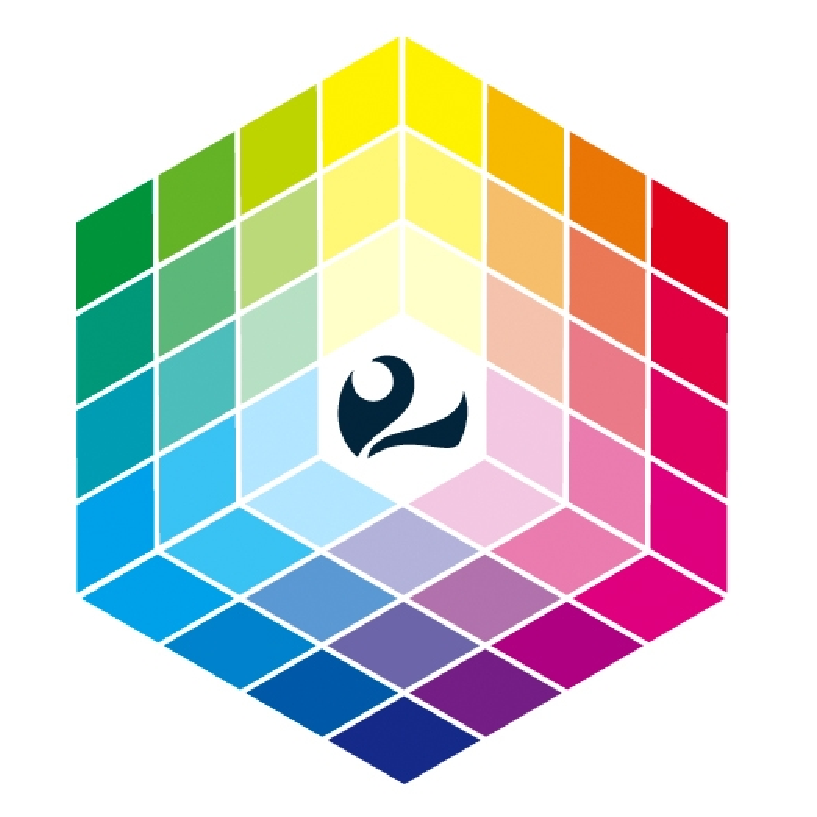
\includegraphics[scale=0.4]{img/logoUm2.eps} \end{center}

\end{frame}



\section{Android}

\subsection{Le système d'exploitation}

\begin{frame}
\frametitle{Android}
\framesubtitle{Le système d'exploitation}
Android est un système basé sur un noyau Linux, développé par Google.
\begin{itemize}
	\item collaboration avec les membres de l'Open Handset Alliance (OHA)
\end{itemize}
\setbeamertemplate{blocks}[rounded,shadow=true]
\begin{block}{OHA}
consortium de compagnie rassemblant leurs compétences pour l'innovation dans le domaine de la mobilité.
\begin{itemize}
	\item Initié par Google en 2007
	\item Opérateur téléphonique, fabricants électroniques, sociétés commerciales
\end{itemize}
\end{block}
\end{frame}

\begin{frame}
\frametitle{Android}
\framesubtitle{Le système d'exploitation}
Structure:
\begin{itemize}
	\item Noyaux linux pour exploiter le matériel
	\item Librairies connues et open source (OpenGL ES, SQLite,...)
	\item Machine virtuelle Java (Dalvik virtual machine)
	\item API Java riche (package de Java SE, open source ou spécifique au système)
\end{itemize}
\end{frame}

\subsection{Développement}

\begin{frame}
\frametitle{Android}
\framesubtitle{Développement}
\begin{itemize}
	\item Langage principale Java, développement en C/C++ possible
	\item Kit de développement multiplateforme
	\item Développement sur téléphone ou sur émulateur
	\item Déploiement des applications peu coûteux
\end{itemize}
\end{frame}

\subsection{Les téléphones mobiles}

\begin{frame}
\frametitle{Android}
\framesubtitle{Les téléphones mobiles}
Les téléphones ont tous l'équipement nécessaire pour la réalité augmentée depuis le premier modèle.\\
\begin{block}{Inconvénient}
\begin{itemize}
	\item Fragmentation des téléphones et des versions du système.
\end{itemize}
\end{block}
%Support des angles de vue de la caméra depuis Android 2.2.\\
%$\Rightarrow$ 70\% des téléphones sous cette version
\end{frame}

\begin{frame}
\frametitle{Android}
\framesubtitle{Les téléphones mobiles}
\begin{block}{Fragmentation}
\begin{itemize}
	\item 7 versions du système en circulation
	\item Différentes dimensions et densités d'écran
	\item Smartphone, tablette (et télévision)
\end{itemize}
\end{block}
\textbf{Besoin:} applications compatibles sur tout les appareils.\\
\textbf{Solution:} compatibilité descendante des applications, système de ressource évolué.
\end{frame}

%\subsection{Structure des applications}

%\begin{frame}
%\frametitle{Android}
%\framesubtitle{Structure des applications}
%\begin{itemize}
%	\item AndroidManifest.xml: déclaration des composant de l'application, des permissions, de la compatibilité, ...
%	\item Ressources: images, descriptions d'interface, texte (multilingue), ...
%	\item Code exécutable: classe Java (package)
%\end{itemize}
%\end{frame}




\section{Application}
\subsection{Lancement de l'application}

	\begin{frame}
	\frametitle{Application}
	\framesubtitle{Ecran de chargement de l'application}
	
	\end{frame}
	
	
	\begin{frame}
	\frametitle{Application}
	\framesubtitle{Ecran d'accueil}
	
	\end{frame}
	
	\begin{frame}
	\frametitle{Application}
	\framesubtitle{Les menus}
	
	\end{frame}
	
\subsection{Editeur de cartes}

	\begin{frame}
	\frametitle{Application}
	\framesubtitle{Gestion des ressources}
	
	
	\end{frame}

	\begin{frame}
	\frametitle{Application}
	\framesubtitle{Création ou chargement d'une carte}
	
	\end{frame}
	
	\begin{frame}
	\frametitle{Application}
	\framesubtitle{Moteur de rendu cartes}
	
	\end{frame}
	
	
	\begin{frame}
	\frametitle{Application}
	\framesubtitle{Editeur de cartes}
	
	\end{frame}
	
	\begin{frame}
	\frametitle{Application}
	\framesubtitle{Outils}
	
	\end{frame}
	
	\begin{frame}
	\frametitle{Application}
	\framesubtitle{Exemple de carte}
	
	\end{frame}
	
	\begin{frame}
	\frametitle{Application}
	\framesubtitle{Possibilités finales}
	
	\end{frame}

\subsection{Jeu}
	
	\begin{frame}
	\frametitle{Application}
	\framesubtitle{Création d'une partie solitaire}
	
		\begin{tabular}{cc}
			\begin{minipage}{5cm}
				Création d'une partie solitaire
				\begin{enumerate}
					\item Choix de la carte
					\item Type de la partie
					\item Difficulté des ennemis
					\item Nombre d'ennemis
					\item Temps de la partie
					\item Retourner à l'écran d'accueil
					\item Créer la partie
				\end{enumerate}
			\end{minipage} &
			\begin{minipage}{7cm}
				\includegraphics[width=6cm]{img/singleplayerbis.png} 
			\end{minipage}\\
		\end{tabular}
	
	\end{frame}
	
	\begin{frame}
	\frametitle{Application}
	\framesubtitle{Intelligence artificielle}
	
		\begin{tabular}{cc}
			\begin{minipage}{4cm}
				Niveaux de difficulté
				\begin{enumerate}
					\item Facile
					\item Moyen
					\item Difficile
				\end{enumerate}
			\end{minipage} &
			\begin{minipage}{6cm}
				\includegraphics[width=6cm]{img/bots.png} 
			\end{minipage}\\
		\end{tabular}
	
	\end{frame}
	
	\begin{frame}
	\frametitle{Application}
	\framesubtitle{Pathfinding}
	
		\begin{tabular}{cc}
			\begin{minipage}{5cm}
				Algorithme A*
				\begin{enumerate}
					\item Heuristique (de Manatan)
					\item Coût de deplacement
					\item Premier chemin trouvé
					\item Rapidité (Dijskra)
				\end{enumerate}
			\end{minipage} &
			\begin{minipage}{5cm}
				\includegraphics[width=6cm]{img/astar.png} 
			\end{minipage}\\
		\end{tabular}
	
	\end{frame}
	
	\begin{frame}
	\frametitle{Application}
	\framesubtitle{Pathfinding}
	
		\begin{tabular}{cc}
			\begin{minipage}{5cm}
				Algorithme de parcours en largeur
				\begin{enumerate}
					\item Pas de case d'arrivé necessaire
					\item Tous les chemins possibles
					\item Premier chemin trouvé
					\item Rapidité
				\end{enumerate}
			\end{minipage} &
			\begin{minipage}{5cm}
							\begin{center}
				\begin{tabular}{|c|c|c|c|c|c|c|} \hline
				\rowcolor{gray}  &  &                    &  &                  &  &                   \\\hline
				\cellcolor{gray} & \cellcolor{orange}1 $\leftarrow$ & \cellcolor{green}1 $\leftarrow$                   &&                && \cellcolor{gray} \\\hline
				\cellcolor{gray} & \cellcolor{orange}1 $\leftarrow$ & \cellcolor{gray}   & \cellcolor{gray} & \cellcolor{gray} &&	\cellcolor{gray} \\\hline
				\cellcolor{gray} & \cellcolor{orange}1 $\leftarrow$ & \cellcolor{orange}1 & \cellcolor{orange}1 $\rightarrow$ & \cellcolor{red}O                 && \cellcolor{gray} \\\hline
				\cellcolor{gray} & \cellcolor{orange}1 $\leftarrow$ & \cellcolor{gray}   & \cellcolor{gray} & \cellcolor{gray} && \cellcolor{gray} \\\hline
				\cellcolor{gray} & \cellcolor{red}O &                  &  &                && \cellcolor{gray} \\\hline
				\cellcolor{gray} && \cellcolor{gray}   && \cellcolor{gray} &&	\cellcolor{gray} \\\hline
				\cellcolor{gray} &&                  &&                && \cellcolor{gray} \\\hline
				\rowcolor{gray}  &  &                    &  &                  &  & \\\hline
				\end{tabular}
			\end{center}
			\end{minipage}\\
		\end{tabular}	
	
	\end{frame}
	
	\begin{frame}
	\frametitle{Application}
	\framesubtitle{Moteur de rendu}
	
		\begin{tabular}{ccccc}
			\begin{minipage}{3cm}
				\begin{center}
					Image
				\end{center}		
			\end{minipage} & &
			\begin{minipage}{2cm}
				\begin{center}
					Hashmap
				\end{center}
			\end{minipage} & &
			\begin{minipage}{3cm}
				\begin{center}
					Resultat
				\end{center}
			\end{minipage}\\
			\begin{minipage}{3cm}
				\includegraphics[width=3cm]{img/bitmap.png}
			\end{minipage} & + &
			\begin{minipage}{2cm}
				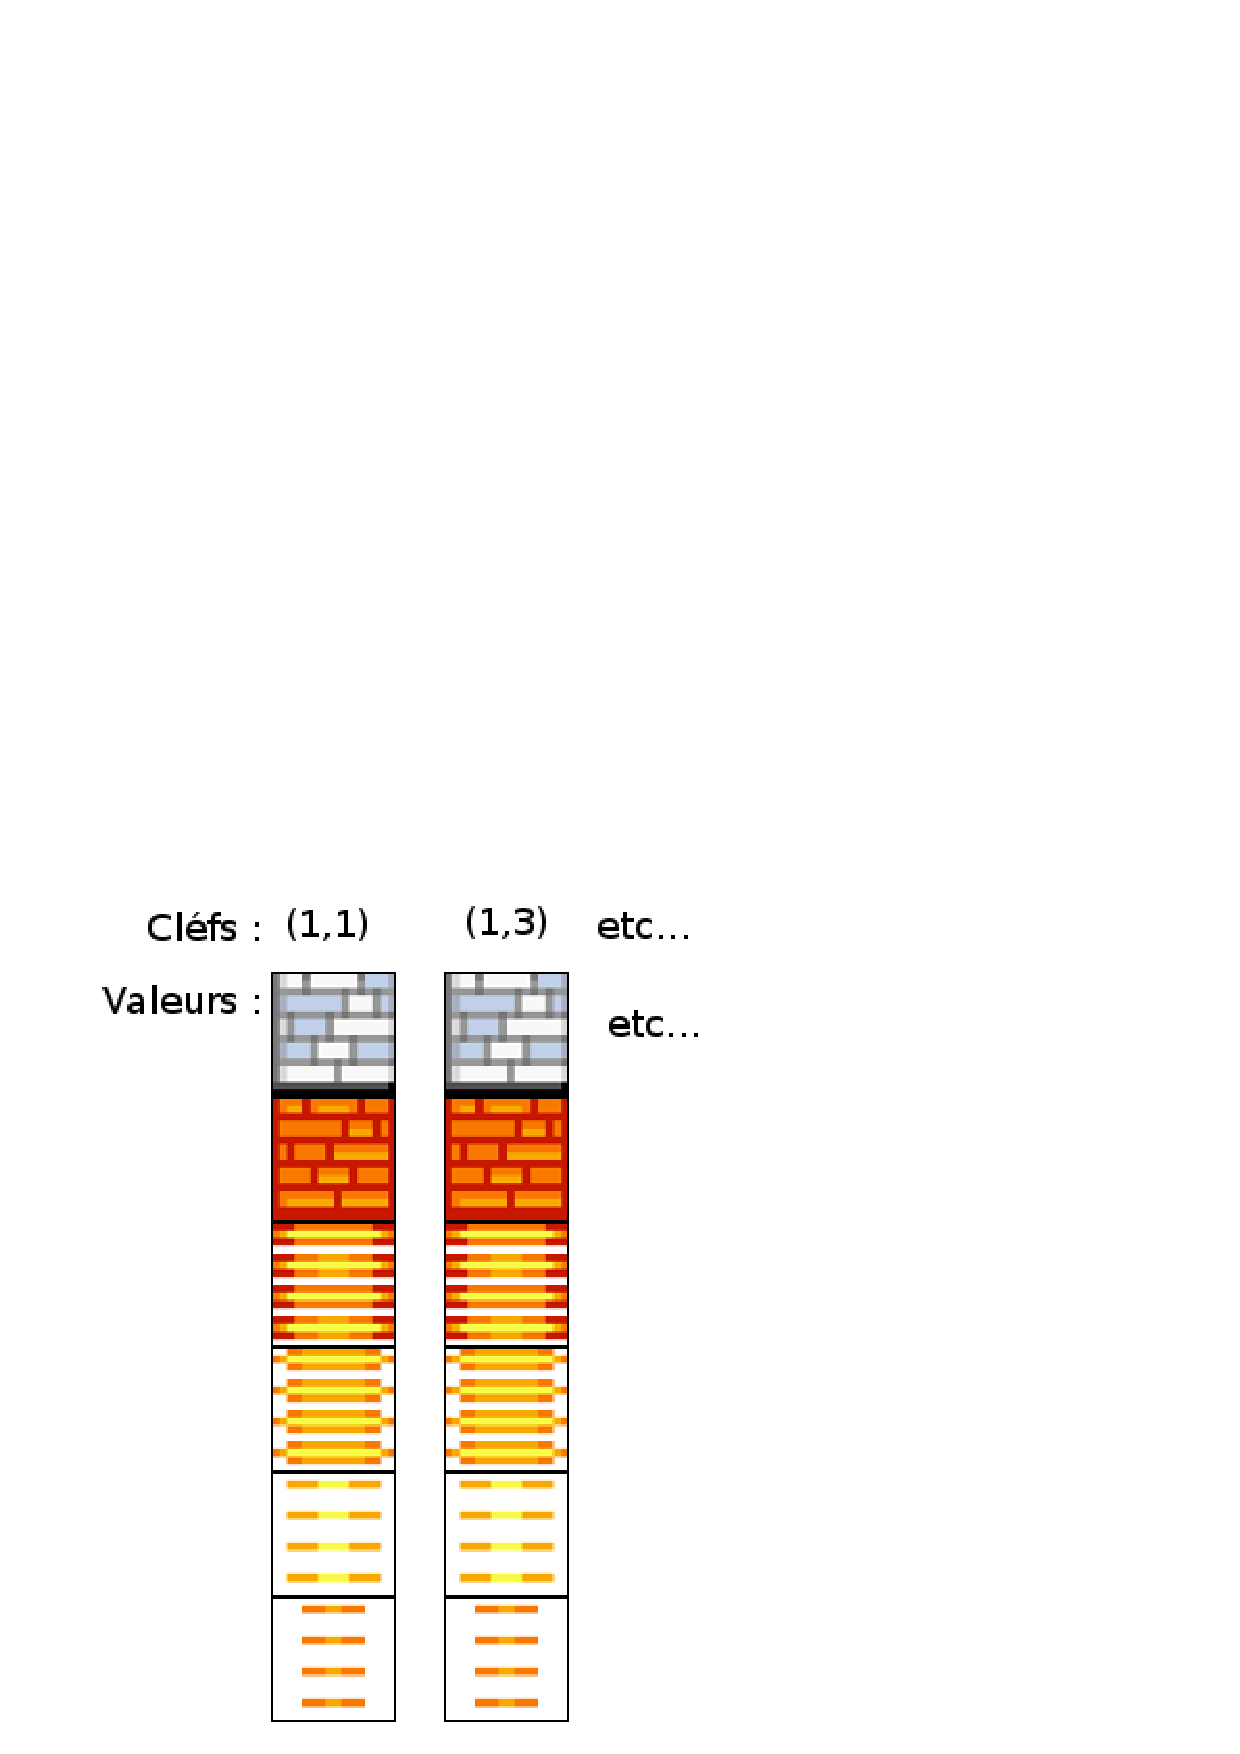
\includegraphics[width=3cm]{img/hashmap.png} 
			\end{minipage} & = &
			\begin{minipage}{3cm}
				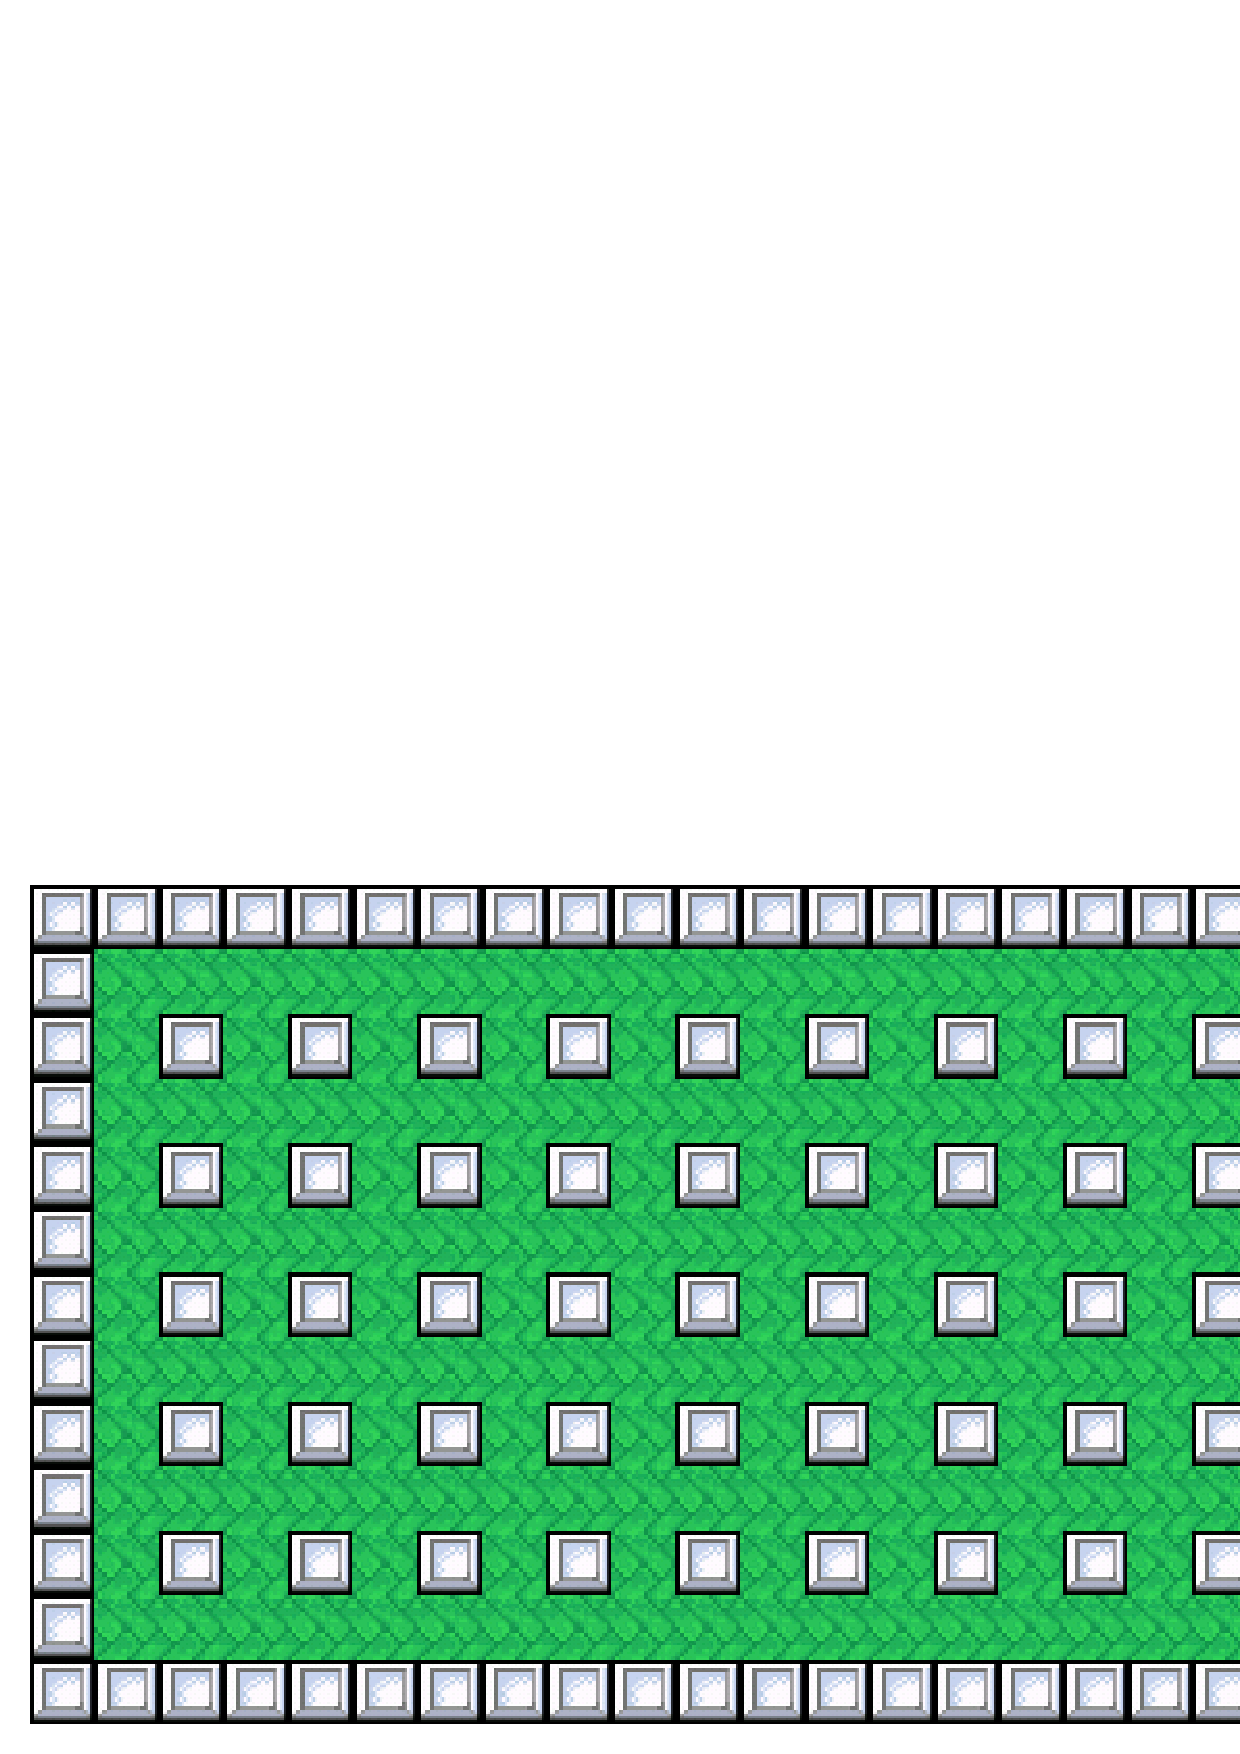
\includegraphics[width=3cm]{img/map.png} 
			\end{minipage}\\
		\end{tabular}
	
	\end{frame}
	
	\begin{frame}
	\frametitle{Application}
	\framesubtitle{Moteur Physique}
	
	\end{frame}
	
	\begin{frame}
	\frametitle{Application}
	\framesubtitle{Multitouch}
	
	\end{frame}
	
	\begin{frame}
	\frametitle{Application}
	\framesubtitle{Menu}
	
			\begin{tabular}{cc}
			\begin{minipage}{4cm}
				Menu
				\begin{enumerate}
					\item Reprendre
					\item Options
					\item Redemarrer
					\item Quitter
				\end{enumerate}
			\end{minipage} &
			\begin{minipage}{7cm}
				\includegraphics[width=7cm]{img/menusolo.png} 
			\end{minipage}\\
		\end{tabular}
	
	\end{frame}


\subsection{Reseau}

\section{Discussion}

	\subsection{Difficultés}
		\begin{frame}
			\frametitle{Discussion}
			\framesubtitle{Difficultés}
				\begin{tabular}{|c|c|c|}
					Android 			 & iOS 					& Serveur \\\hline
					\multicolumn{2}{|c|}{Ressources limitées} 	& Déploiement local\\	
					\multicolumn{2}{|c|}{Nouvelle plate-forme}	& Servlets \\
										 & Nouveau langage  	& Communication avec \\
										 & (Objective-C) 		& la base de données\\
					 Multi-touch		 & 						& \\
						  				 & Gestion manuelle 	& \\
						  				 & de la mémoire 		& \\
			\end{tabular}
		\end{frame}
		
		
	\subsection{Problèmes}
		\begin{frame}
			\frametitle{Discussion}
			\framesubtitle{Problèmes}
			Android et iOS :
			\begin{itemize}
				\item Tester l'application
				\item OpenGL ES
			\end{itemize}
			
			Serveur :
			\begin{itemize}
				\item Déploiement internet
			\end{itemize}
						
		\end{frame}
		
		
	\subsection{Améliorations}
		\begin{frame}
			\frametitle{Discussion}
			\framesubtitle{Améliorations}
			\begin{itemize}
				\item Mode histoire
				\item Ajout de bonus / malus
				\item Rajout de types de parties
				\item Gestion des scores
				\item Nouvelles bombes
			\end{itemize}
		\end{frame}


\section{Conclusion}

\begin{frame}
\frametitle{Conclusion}
\framesubtitle{Ce que cela nous a apporté}
\begin{itemize}
	\item Découverte de la programmation mobile (SDK Android)
	\item Notion de réalité augmentée
	\item Utilisation de la géolocalisation via les smartphones
\end{itemize}
\end{frame}



\end{document}
